% sub-subsetion for 4.2.2 ----- ESTRATEGIA DE BUSQUEDA POR SNOWBALL
\subsubsection{Estrategia de Búsqueda 2: Bola de nieve}

\newcommand{\firstBackwardSnowballStudies}{8} %Primera iteración hacia atrás
\newcommand{\firstForwardSnowballStudies}{7} % Primera iteración hacia adelante

%Total de estudios
\newcommand{\snowballNewStudies}{\fpeval{\firstBackwardSnowballStudies+\firstForwardSnowballStudies}}

La estrategia de búsqueda mediante \textit{snowballing} se aplicó con el objetivo de identificar estudios adicionales que pudieran 
no haber sido recuperados durante la búsqueda automática en las bases de datos. Siguiendo las recomendaciones metodológicas de 
Wohlin~\cite{Wohlin-01}, se consideraron tanto la bola de nieve inversa, basada en el análisis de las listas de referencias de los 
estudios seleccionados, como la bola de nieve directa, que consiste en identificar los trabajos que citan dichos estudios. Para este 
propósito se utilizó Google Académico como motor de búsqueda para el rastreo de citas.

% Snowball baseline building 
\bolditalic{Construcción de la base de la bola de nieve}: 
Como diferenciador metodológico, en este trabajo la estrategia de \textit{snowballing} se aplicó sobre la totalidad de los 166 
estudios seleccionados tras el proceso de selección, en lugar de emplear un conjunto reducido de artículos base (semilla). Esta 
decisión permitió ampliar la cobertura de la revisión y disminuir el riesgo de omitir literatura relevante, fortaleciendo la 
exhaustividad del protocolo.

\bolditalic{Selección de estudios}: 
A partir de los 166 estudios semilla se aplicaron las estrategias de bola de nieve directa e inversa con el objetivo de identificar 
literatura adicional relevante que no hubiera sido recuperada durante la búsqueda automática en las bases de datos. Los estudios 
identificados mediante este proceso fueron evaluados aplicando los mismos criterios de inclusión y exclusión definidos en la 
Tabla~\ref{table:inclusion_exclusion_criteria}, garantizando así la consistencia y rigurosidad del proceso de selección dentro del 
estudio de mapeo sistemático.

\begin{figure}[htbp]
	\centering
	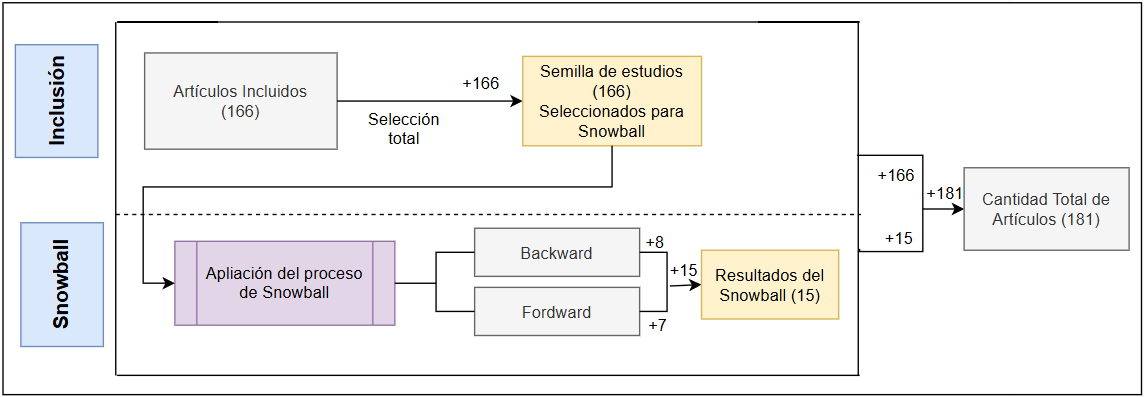
\includegraphics[scale=0.30]{resources/images/Planeacion/proceso_snowball.png}
	\caption{Estrategica de Busqueda Snowball.}\label{figure:Snowball}
\end{figure}

Esta actividad se realizó a través de Google Scholar, siguiendo la práctica del estudio~\cite{Ali-01}. El resultado obtenido fue 
\snowballNewStudies{} nuevos estudios. Cabe destacar que lo presentado en esta sección y en la Figura\ref{figure:Snowball} es un resumen 
representativo del proceso de bola de nieve; sin embargo, se omiten los pasos realizados que no contribuyen al objetivo del estudio. 
Por ejemplo, durante el proceso de bola de nieve se identificaron estudios que no cumplían con los criterios de inclusión, como libros y 
duplicados. Estos estudios fueron descartados y no se incluyeron en el conteo final de nuevos estudios obtenidos a través del proceso de 
bola de nieve.

% -------- Table : Inclusion/exclusion criteria ------------
\begin{table}[htbp]
	\centering
	\renewcommand{\arraystretch}{1}  % Increase row height globally
	\begin{tabular}{p{1.5cm}p{2.2cm}p{3.9cm}}
		\toprule
		\textbf{Category}         & \textbf{Inclusion} & \textbf{Exclusion}                                                                                           \\
		\midrule
		\textbf{Publication type} & Journal articles, Chapters  & Technical report, Conference proceedings and Thesis. \\
		\addlinespace[0.8em]
		\textbf{Period}           & From 2020 to 2026  & Less than 2020                                                                                                \\
		\addlinespace[0.8em]
		\textbf{Language}         & English            & ---                                                                                                              \\
		\bottomrule
		\vspace{1pt}
	\end{tabular}
	\caption{Criterios de Inclusion/exclusion Snowball}\label{table:inclusion_exclusion_criteria}
\end{table}
% --------------------------------------------------------------